\documentclass{article}
\usepackage[utf8]{inputenc}
\usepackage{ctex}
\usepackage{amsmath, amssymb, amsfonts}
\usepackage{geometry}
\usepackage{booktabs}
\usepackage{titlesec}
\usepackage{enumitem}
\usepackage{pgfplots}
\pgfplotsset{compat=1.18}
\usepgfplotslibrary{fillbetween}
\definecolor{myblue}{RGB}{30, 100, 170}
\definecolor{myred}{RGB}{200, 50, 50}
\definecolor{mygreen}{RGB}{50, 130, 50}

% 页面边距优化
\geometry{top=2.5cm, bottom=2.5cm, left=2.5cm, right=2.5cm}

% 章节样式美化
\titleformat{\section}{\large\bfseries}{\thesection.}{0.5em}{}
\titleformat{\subsection}{\normalsize\bfseries}{\thesubsection}{0.5em}{}

% 取消首行缩进并设置段落间距
\setlength{\parindent}{0pt}
\setlength{\parskip}{0.5em}

\title{\textbf{高等数学核心基础知识点速查手册}}
\author{25级哲学班\textbf{阿苏塔卡}}
\date{}

\begin{document}

\maketitle
\thispagestyle{empty} % 首页不显示页码

\section{三角函数与反三角函数基本知识}
\subsection{六大基本三角函数定义与性质}
在直角坐标系中，设角 $\alpha$ 终边上任意一点为 $P(x, y)$，其到原点的距离为 $r = \sqrt{x^2+y^2}$。
\begin{itemize}[leftmargin=1.5em, itemsep=0.1em]
    \item \textbf{正弦 ($\sin\alpha$):} $\frac{y}{r}$，定义域 $\mathbb{R}$，值域 $[-1, 1]$，周期 $2\pi$，奇函数。
    \item \textbf{余弦 ($\cos\alpha$):} $\frac{x}{r}$，定义域 $\mathbb{R}$，值域 $[-1, 1]$，周期 $2\pi$，偶函数。
    \item \textbf{正切 ($\tan\alpha$):} $\frac{y}{x}$，定义域 $\left\{x \mid x \neq k\pi + \frac{\pi}{2}, k \in \mathbb{Z}\right\}$调，值域 $\mathbb{R}$，周期 $\pi$，奇函数。
    \item \textbf{余切 ($\cot\alpha$):} $\frac{x}{y}$，定义域 $\{x \mid x \neq k\pi, k \in \mathbb{Z}\}$，值域 $\mathbb{R}$，周期 $\pi$，奇函数。
    \item \textbf{正割 ($\sec\alpha$):} $\frac{r}{x} = \frac{1}{\cos\alpha}$，定义域 $\left\{x \mid x \neq k\pi + \frac{\pi}{2}, k \in \mathbb{Z}\right\}$，值域 $(-\infty, -1] \cup [1, +\infty)$。
    \item \textbf{余割 ($\csc\alpha$):} $\frac{r}{y} = \frac{1}{\sin\alpha}$，定义域 $\{x \mid x \neq k\pi, k \in \mathbb{Z}\}$，值域 $(-\infty, -1] \cup [1, +\infty)$。
\end{itemize}
\subsection{三角函数的图像}
% 第一组：正弦与余弦
\begin{minipage}{0.48\textwidth}
    \centering
    \begin{tikzpicture}[scale=0.7]
        \begin{axis}[
            axis lines = middle,
            xlabel = $x$, ylabel = $y$,
            xmin = -6.5, xmax = 6.5,
            ymin = -1.5, ymax = 1.5,
            xtick = {-6.28, -3.14, 0, 3.14, 6.28},
            xticklabels = {$-2\pi$, $-\pi$, 0, $\pi$, $2\pi$},
            grid = both, grid style = {dashed, gray!30},
            title = {$\sin x$ (蓝) 与 $\cos x$ (红)},
            legend style={at={(0.5,-0.2)},anchor=north,legend columns=-1}
        ]
            \addplot [domain=-2*pi:2*pi, samples=100, thick, myblue] {sin(deg(x))};
            \addplot [domain=-2*pi:2*pi, samples=100, thick, myred] {cos(deg(x))};
        \end{axis}
    \end{tikzpicture}
\end{minipage}
\hfill
% 第二组：正切与余切
\begin{minipage}{0.48\textwidth}
    \centering
    \begin{tikzpicture}[scale=0.7]
        \begin{axis}[
            axis lines = middle,
            xlabel = $x$, ylabel = $y$,
            xmin = -4, xmax = 4,
            ymin = -4, ymax = 4,
            xtick = {-3.14, -1.57, 0, 1.57, 3.14},
            xticklabels = {$-\pi$, $-\frac{\pi}{2}$, 0, $\frac{\pi}{2}$, $\pi$},
            grid = both, grid style = {dashed, gray!30},
            title = {$\tan x$ (蓝) 与 $\cot x$ (红)},
            restrict y to domain=-10:10
        ]
            \addplot [domain=-1.4:1.4, samples=50, thick, myblue] {tan(deg(x))};
            \addplot [domain=1.7:3.1, samples=50, thick, myblue] {tan(deg(x))};
            \addplot [domain=-3.1:-1.7, samples=50, thick, myblue] {tan(deg(x))};
            \addplot [domain=0.1:3, samples=50, thick, myred] {1/tan(deg(x))};
            \addplot [domain=-3:-0.1, samples=50, thick, myred] {1/tan(deg(x))};
        \end{axis}
    \end{tikzpicture}
\end{minipage}

\vspace{1em}

% 第三组：正割与余割
\begin{minipage}{0.48\textwidth}
    \centering
    \begin{tikzpicture}[scale=0.7]
        \begin{axis}[
            axis lines = middle,
            xmin = -4, xmax = 4, ymin = -4, ymax = 4,
            grid = both, grid style = {dashed, gray!30},
            title = {$\sec x$ (蓝) 与 $\csc x$ (红)},
            restrict y to domain=-10:10
        ]
            \addplot [domain=-1.4:1.4, samples=50, thick, myblue] {1/cos(deg(x))};
            \addplot [domain=0.2:3, samples=50, thick, myred] {1/sin(deg(x))};
        \end{axis}
    \end{tikzpicture}
\end{minipage}
\hfill
\begin{minipage}{0.48\textwidth}
    \small
    \textbf{核心公式回顾：}
    \begin{itemize}[leftmargin=1em, itemsep=0pt]
        \item $\sin^2 x + \cos^2 x = 1$
        \item $1 + \tan^2 x = \sec^2 x$
        \item $\sin 2x = 2\sin x \cos x$
        \item $\cos 2x = 2\cos^2 x - 1 = 1 - 2\sin^2 x$
    \end{itemize}
\end{minipage}

\section{反三角函数图像}

\begin{minipage}{0.32\textwidth}
    \centering
    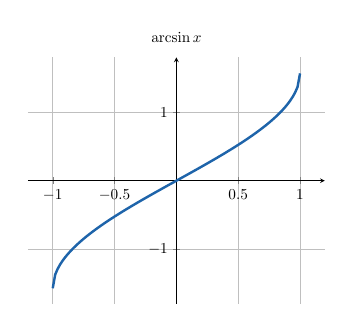
\begin{tikzpicture}[scale=0.55]
        \begin{axis}[axis lines=middle, title={$\arcsin x$}, xmin=-1.2, xmax=1.2, ymin=-1.8, ymax=1.8, grid=both]
            \addplot [domain=-1:1, samples=100, ultra thick, myblue] {asin(x)*pi/180};
        \end{axis}
    \end{tikzpicture}
\end{minipage}
\hfill
\begin{minipage}{0.32\textwidth}
    \centering
    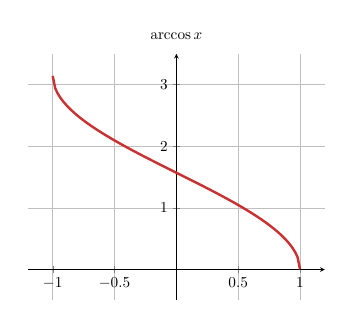
\begin{tikzpicture}[scale=0.55]
        \begin{axis}[axis lines=middle, title={$\arccos x$}, xmin=-1.2, xmax=1.2, ymin=-0.5, ymax=3.5, grid=both]
            \addplot [domain=-1:1, samples=100, ultra thick, myred] {acos(x)*pi/180};
        \end{axis}
    \end{tikzpicture}
\end{minipage}
\hfill
\begin{minipage}{0.32\textwidth}
    \centering
    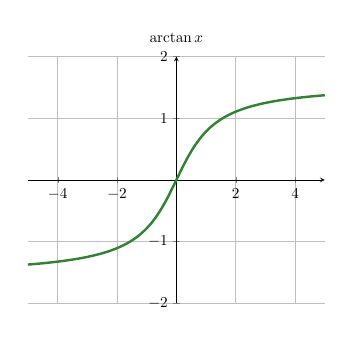
\begin{tikzpicture}[scale=0.55]
        \begin{axis}[axis lines=middle, title={$\arctan x$}, xmin=-5, xmax=5, ymin=-2, ymax=2, grid=both]
            \addplot [domain=-5:5, samples=100, ultra thick, mygreen] {atan(x)*pi/180};
        \end{axis}
    \end{tikzpicture}
\end{minipage}

\subsection{核心三角恒等式}
\begin{itemize}[leftmargin=1.5em]
    \item \textbf{同角平方关系:} $\sin^2 x + \cos^2 x = 1$ \quad,\quad $1 + \tan^2 x = \sec^2 x$ \quad,\quad $1 + \cot^2 x = \csc^2 x$
    \item \textbf{两角和差公式:} 
    \[ \sin(x \pm y) = \sin x \cos y \pm \cos x \sin y \]
    \[ \cos(x \pm y) = \cos x \cos y \mp \sin x \sin y \]
    \[ \tan(x \pm y) = \frac{\tan x \pm \tan y}{1 \mp \tan x \tan y} \]
    \item \textbf{二倍角公式:} 
    \[ \sin 2x = 2\sin x \cos x \]
    \[ \cos 2x = \cos^2 x - \sin^2 x = 2\cos^2 x - 1 = 1 - 2\sin^2 x \]
    \item \textbf{降幂公式 (高数求积分常用):} 
    \[ \sin^2 x = \frac{1 - \cos 2x}{2} \quad,\quad \cos^2 x = \frac{1 + \cos 2x}{2} \]
\end{itemize}

\subsection{三大反三角函数}
反三角函数是严格受限区间上的逆运算：
\begin{itemize}[leftmargin=1.5em, itemsep=0.1em]
    \item \textbf{反正弦 ($\arcsin x$):} 定义域 $[-1, 1]$，值域 $\left[-\frac{\pi}{2}, \frac{\pi}{2}\right]$，奇函数。
    \item \textbf{反余弦 ($\arccos x$):} 定义域 $[-1, 1]$，值域 $[0, \pi]$，非奇非偶函数，满足 $\arcsin x + \arccos x = \frac{\pi}{2}$。
    \item \textbf{反正切 ($\arctan x$):} 定义域 $\mathbb{R}$，值域 $\left(-\frac{\pi}{2}, \frac{\pi}{2}\right)$，奇函数，极限满足 $\lim_{x \to +\infty} \arctan x = \frac{\pi}{2}$，$\lim_{x \to -\infty} \arctan x = -\frac{\pi}{2}$。
\end{itemize}
\section{等价无穷小基本知识}

\subsection{定义与性质}
设在某一极限过程中，$\alpha(x) \to 0$ 且 $\beta(x) \to 0$。若 $\lim \frac{\alpha(x)}{\beta(x)} = 1$，则称 $\alpha(x)$ 与 $\beta(x)$ 是该过程中的\textbf{等价无穷小}，记作 $\alpha(x) \sim \beta(x)$。
\begin{itemize}[leftmargin=1.5em]
    \item \textbf{乘积代换定理:} 若 $\alpha \sim \alpha'$, $\beta \sim \beta'$，则 $\lim \frac{\alpha \cdot \beta}{\gamma} = \lim \frac{\alpha' \cdot \beta'}{\gamma}$（因式中的无穷小可直接代换）。
    \item \textbf{加减代换警告:} 加减法中通常不能随意代换，除非 $\alpha \sim \alpha'$ 且 $\beta \sim \beta'$ 时，满足 $\lim \frac{\alpha'}{\beta'} \neq 1$（即两者不是同阶无穷小相减）。通常建议使用泰勒公式处理加减法中的无穷小。
\end{itemize}

\subsection{常用等价无穷小公式 (当 $x \to 0$ 时)}
以下是微积分求极限最常用的等价无穷小关系：
\begin{table}[h]
\centering
\begin{tabular}{lcl}
\toprule
\textbf{原函数} & & \textbf{等价无穷小 ($x \to 0$)} \\
\midrule
$\sin x$ & $\sim$ & $x$ \\
$\tan x$ & $\sim$ & $x$ \\
$\arcsin x$ & $\sim$ & $x$ \\
$\arctan x$ & $\sim$ & $x$ \\
$1 - \cos x$ & $\sim$ & $\frac{1}{2}x^2$ \\
$\tan x - \sin x$ & $\sim$ & $\frac{1}{2}x^3$ \\
$e^x - 1$ & $\sim$ & $x$ \\
$a^x - 1$ & $\sim$ & $x \ln a$ \\
$\ln(1 + x)$ & $\sim$ & $x$ \\
$\log_a(1 + x)$ & $\sim$ & $\frac{x}{\ln a}$ \\
$(1 + x)^\alpha - 1$ & $\sim$ & $\alpha x$ \\
\bottomrule
\end{tabular}
\end{table}

\section{函数的间断点基本知识}

\subsection{连续的定义与间断点的产生}
若 $\lim_{x \to x_0} f(x) = f(x_0)$，则称函数 $f(x)$ 在 $x_0$ 处连续。若满足以下三个条件之一，则 $x_0$ 为\textbf{间断点}：
1) $f(x)$ 在 $x_0$ 处无定义；2) $\lim_{x \to x_0} f(x)$ 不存在；3) $\lim_{x \to x_0} f(x) \neq f(x_0)$。

\subsection{间断点的分类}
间断点根据\textbf{左右极限是否存在}分为第一类和第二类。设 $f(x_0^-)$ 为左极限，$f(x_0^+)$ 为右极限。

\subsubsection{第一类间断点 (左右极限均存在)}
\begin{itemize}[leftmargin=1.5em]
    \item \textbf{可去间断点:} $f(x_0^-) = f(x_0^+)$，但该极限不等于 $f(x_0)$（或 $f(x_0)$ 无定义）。可以通过补充或修改该点定义使函数连续。
    \item \textbf{跳跃间断点:} $f(x_0^-) \neq f(x_0^+)$。两者的差值 $|f(x_0^+) - f(x_0^-)|$ 称为函数的跳跃度。
\end{itemize}

\subsubsection{第二类间断点 (左右极限至少有一个不存在)}
\begin{itemize}[leftmargin=1.5em]
    \item \textbf{无穷间断点:} 当 $x \to x_0$ 时，$f(x) \to \infty$。例如 $f(x) = \frac{1}{x}$ 在 $x = 0$ 处。
    \item \textbf{振荡间断点:} 当 $x \to x_0$ 时，函数值在某些值之间无限次变动，极限不存在。例如 $f(x) = \sin\frac{1}{x}$ 在 $x = 0$ 处。
\end{itemize}
\section{基本求导公式表 (必背)}
\begin{table}[h]
\centering\small
\begin{tabular}{ll|ll}
\toprule
\textbf{函数 $f(x)$} & \textbf{导数 $f'(x)$} & \textbf{函数 $f(x)$} & \textbf{导数 $f'(x)$} \\
\midrule
$C$ (常数) & $0$ & $x^n$ & $n x^{n-1}$ \\
$e^x$ & $e^x$ & $a^x$ & $a^x \ln a$ \\
$\ln x$ & $\frac{1}{x}$ & $\log_a x$ & $\frac{1}{x \ln a}$ \\
\midrule
$\sin x$ & $\cos x$ & $\cos x$ & $-\sin x$ \\
$\tan x$ & $\sec^2 x$ & $\cot x$ & $-\csc^2 x$ \\
$\sec x$ & $\sec x \tan x$ & $\csc x$ & $-\csc x \cot x$ \\
\midrule
$\arcsin x$ & $\frac{1}{\sqrt{1-x^2}}$ & $\arccos x$ & $-\frac{1}{\sqrt{1-x^2}}$ \\
$\arctan x$ & $\frac{1}{1+x^2}$ & $\text{arccot}\,x$ & $-\frac{1}{1+x^2}$ \\
\bottomrule
\end{tabular}
\end{table}
\end{document}